\documentclass{beamer}
\usepackage[utf8]{inputenc}
\usepackage{graphicx}

\usetheme{Madrid}
\usecolortheme{default}

%------------------------------------------------------------
%This block of code defines the information to appear in the
%Title page
\title{Multi-armed bandit problem}

\subtitle{}

\author{}

\institute % (optional)
{}

\date % (optional)
{}


%End of title page configuration block
%------------------------------------------------------------


%------------------------------------------------------------
%The next block of commands puts the table of contents at the
%beginning of each section and highlights the current section:

\AtBeginSection[]
{
    \begin{frame}
        \frametitle{Table of Contents}
        \tableofcontents[currentsection]
    \end{frame}
}
%------------------------------------------------------------


\begin{document}

%---------------------------------------------------------
%Changing visivility of the text
    \begin{frame}
        \frametitle{Simulations for Stationary Multi-Armed Bandit Problem}
        Figure 1
        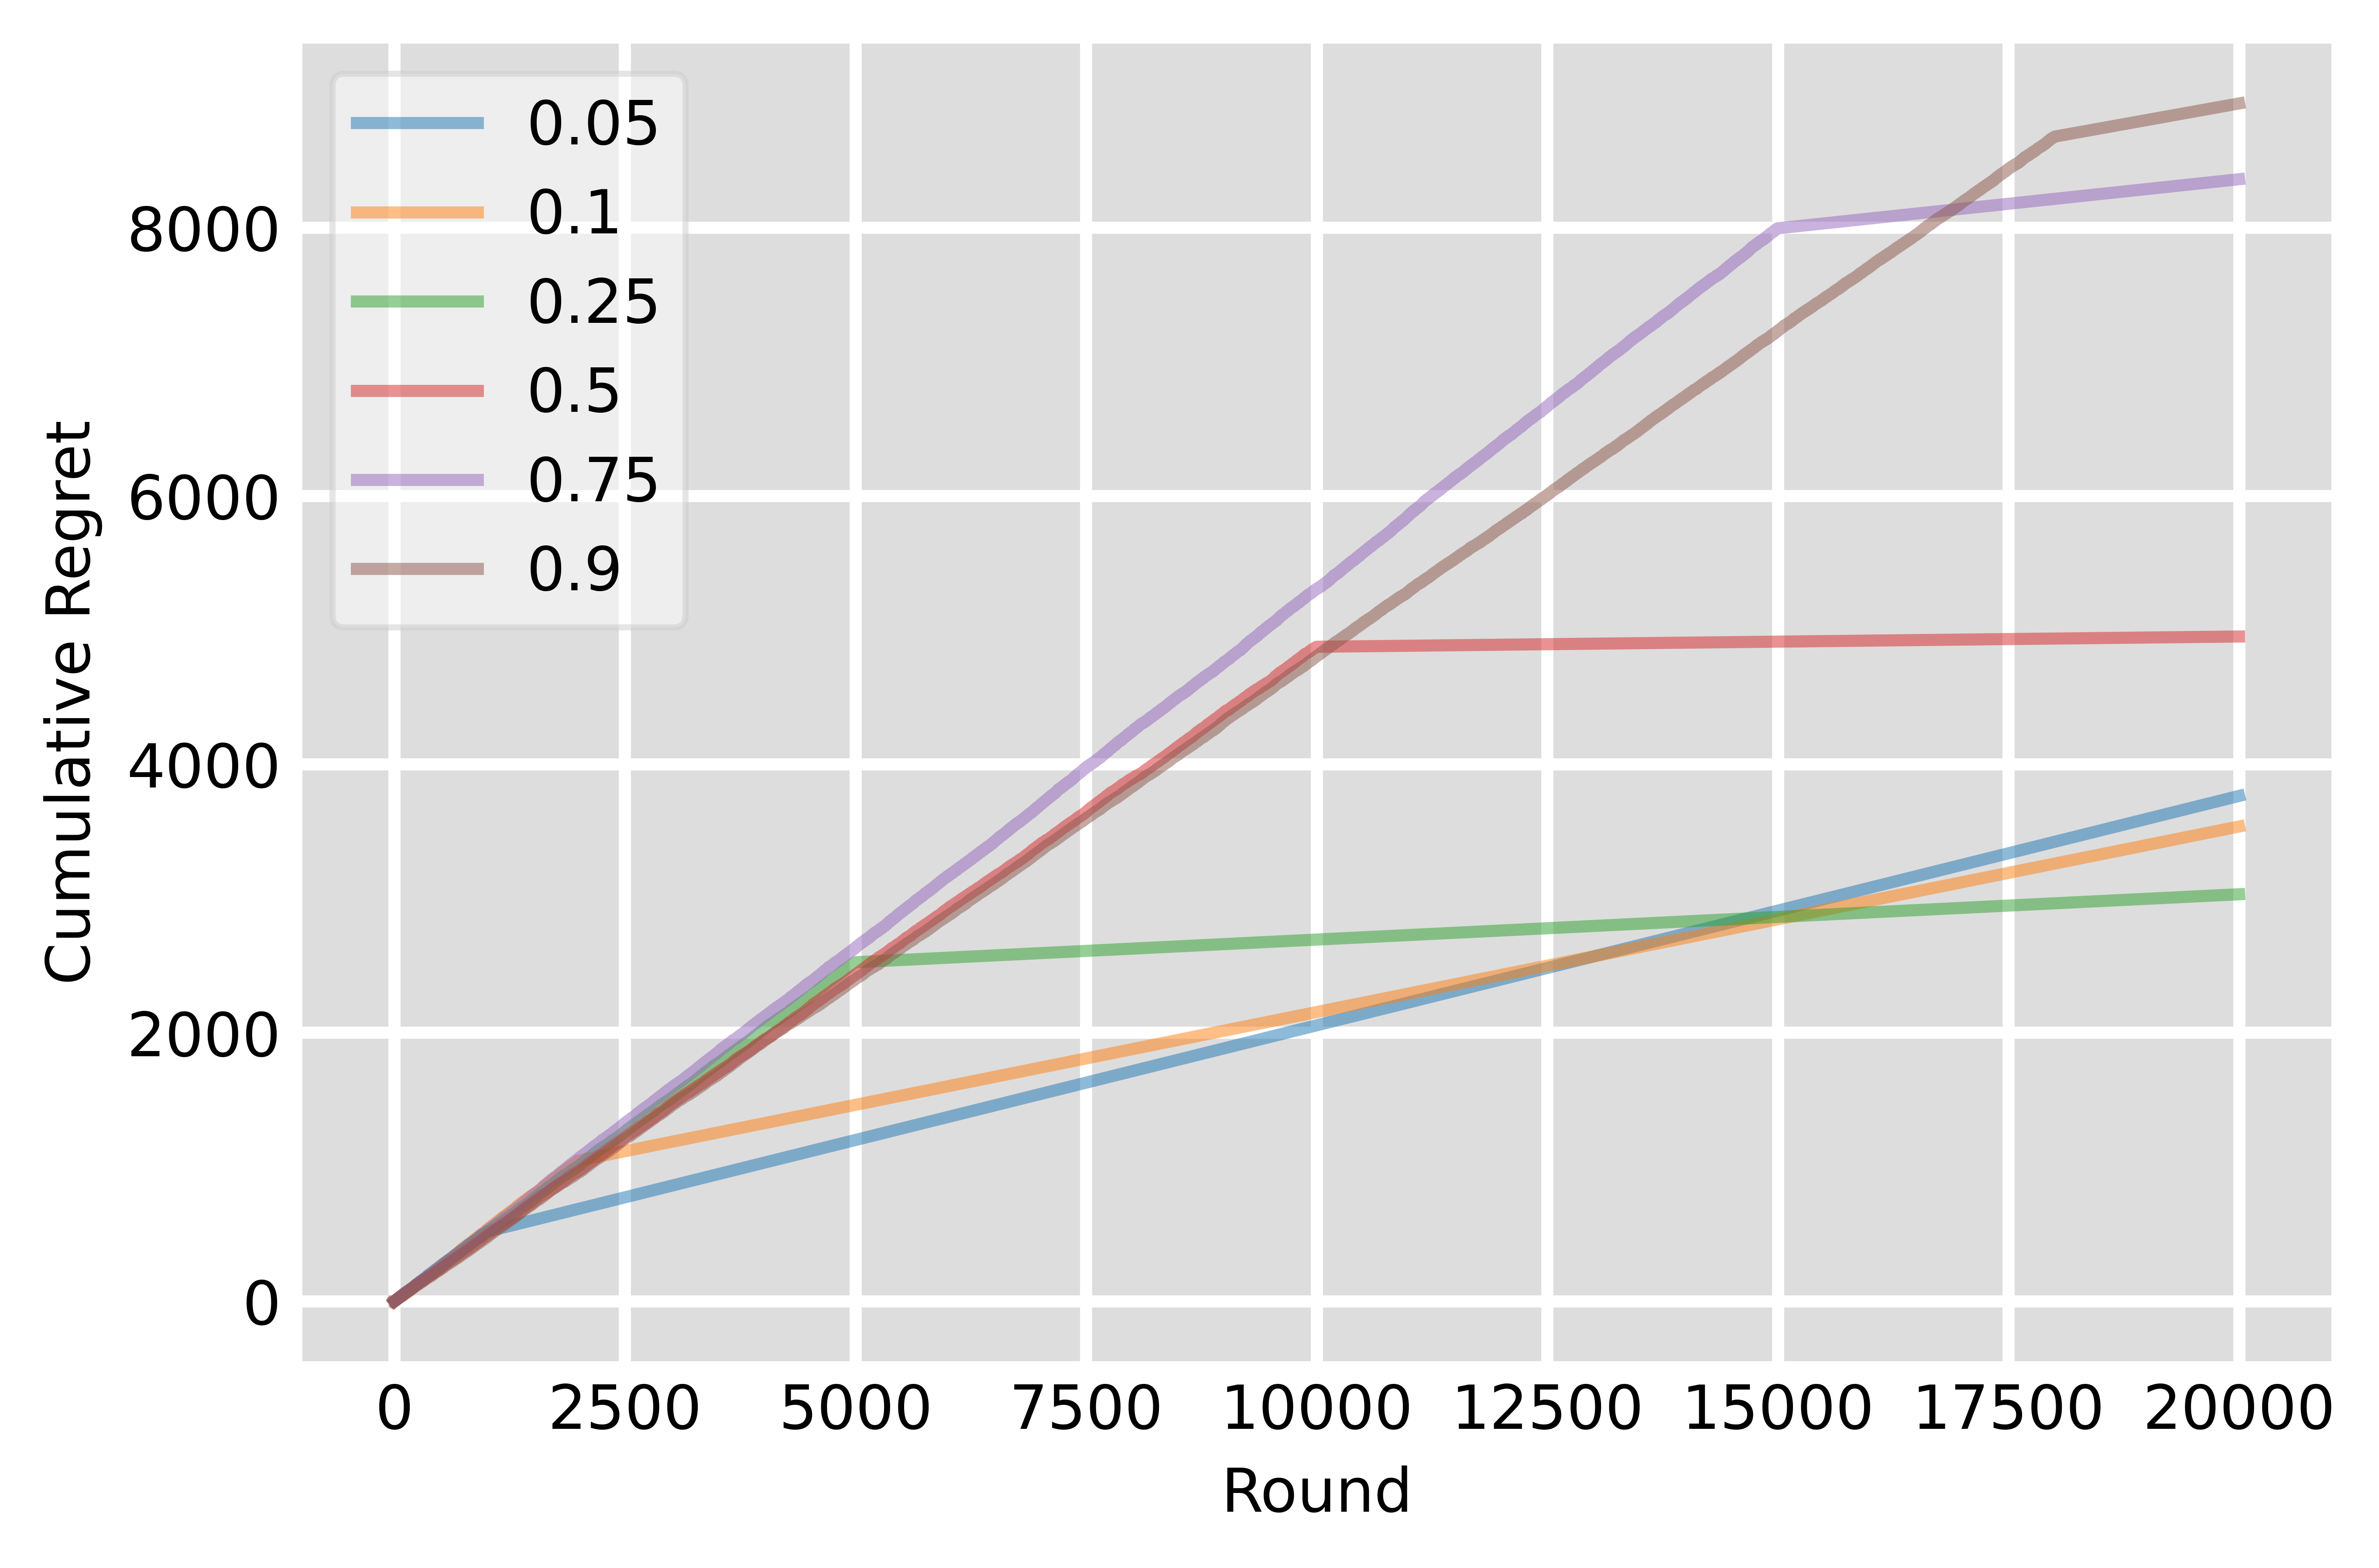
\includegraphics[width=0.9\textwidth]{../report/figures/epsilon_plot.png}
    \end{frame}


\end{document}